% !TEX root = ../main.tex
% ══════════════════════════════════════════════════════════════
%  ANNEXES — partie autonome, distincte des chapitres.
%  Aucune entrée de niveau section/subsection dans la table des
%  matières : seule « Annexes » apparaît, au niveau chapitre.
% ══════════════════════════════════════════════════════════════
\stopcontents[chapters]% clôt la mini-table des matières du dernier chapitre
\cleardoublepage
\phantomsection
\addcontentsline{toc}{chapter}{Annexes}
\markboth{Annexes}{Annexes}

{\centering \Huge\bfseries Annexes \par}
\vspace{2em}

% Numérotation des figures / tableaux d'annexe en « A.n »
\renewcommand{\thefigure}{A.\arabic{figure}}
\renewcommand{\thetable}{A.\arabic{table}}
\setcounter{figure}{0}
\setcounter{table}{0}

\noindent{\large\bfseries Annexe A~--- Captures d'écran complémentaires du chapitre~\ref{cha:realisation}}
\par\medskip
\justifying

Cette annexe regroupe les captures d'écran illustratives qui complètent la
réalisation présentée au chapitre~\ref{cha:realisation}. Pour chaque sprint,
le corps du rapport conserve la capture la plus représentative du résultat
livré ; les vues secondaires, souvent proches visuellement, sont reportées ici.

\bigskip
\noindent\textbf{A.1~--- Sprint 3 : supervision et statistiques d'affectation}
\par\smallskip

\begin{figure}[H]
  \centering
  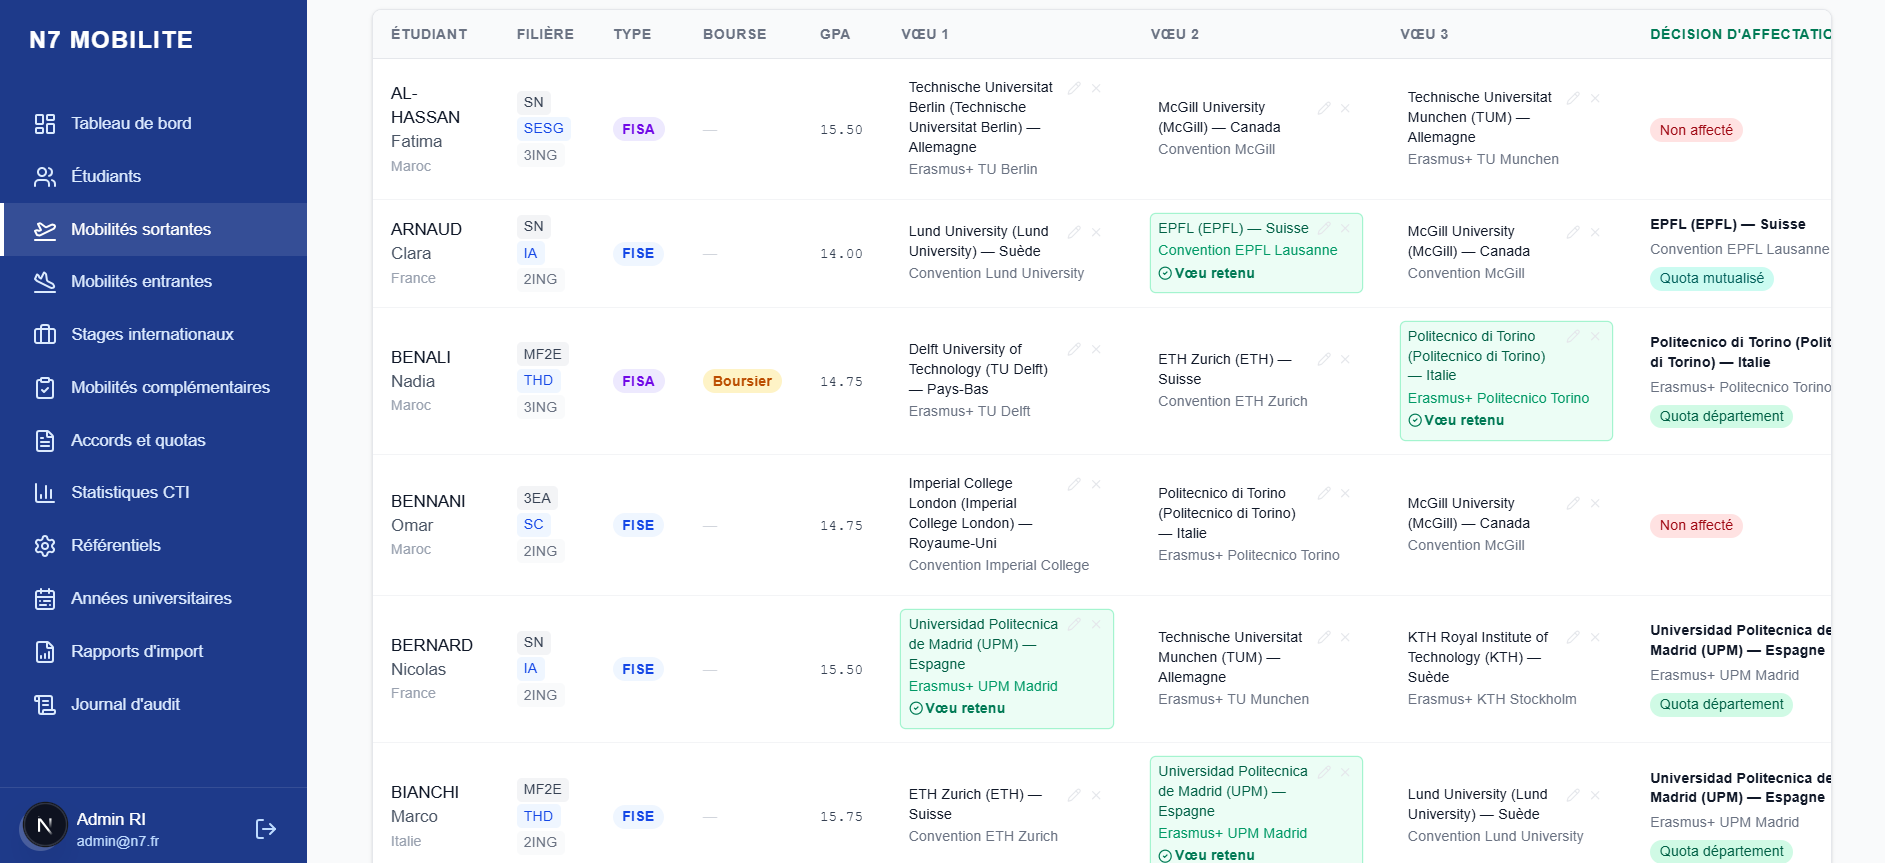
\includegraphics[width=\linewidth]{figures/captures/sprint3/sprint3-supervision.png}
  \caption{Supervision individuelle des propositions d'affectation}
  \label{fig:cap-sprint3-supervision}
\end{figure}

\begin{figure}[H]
  \centering
  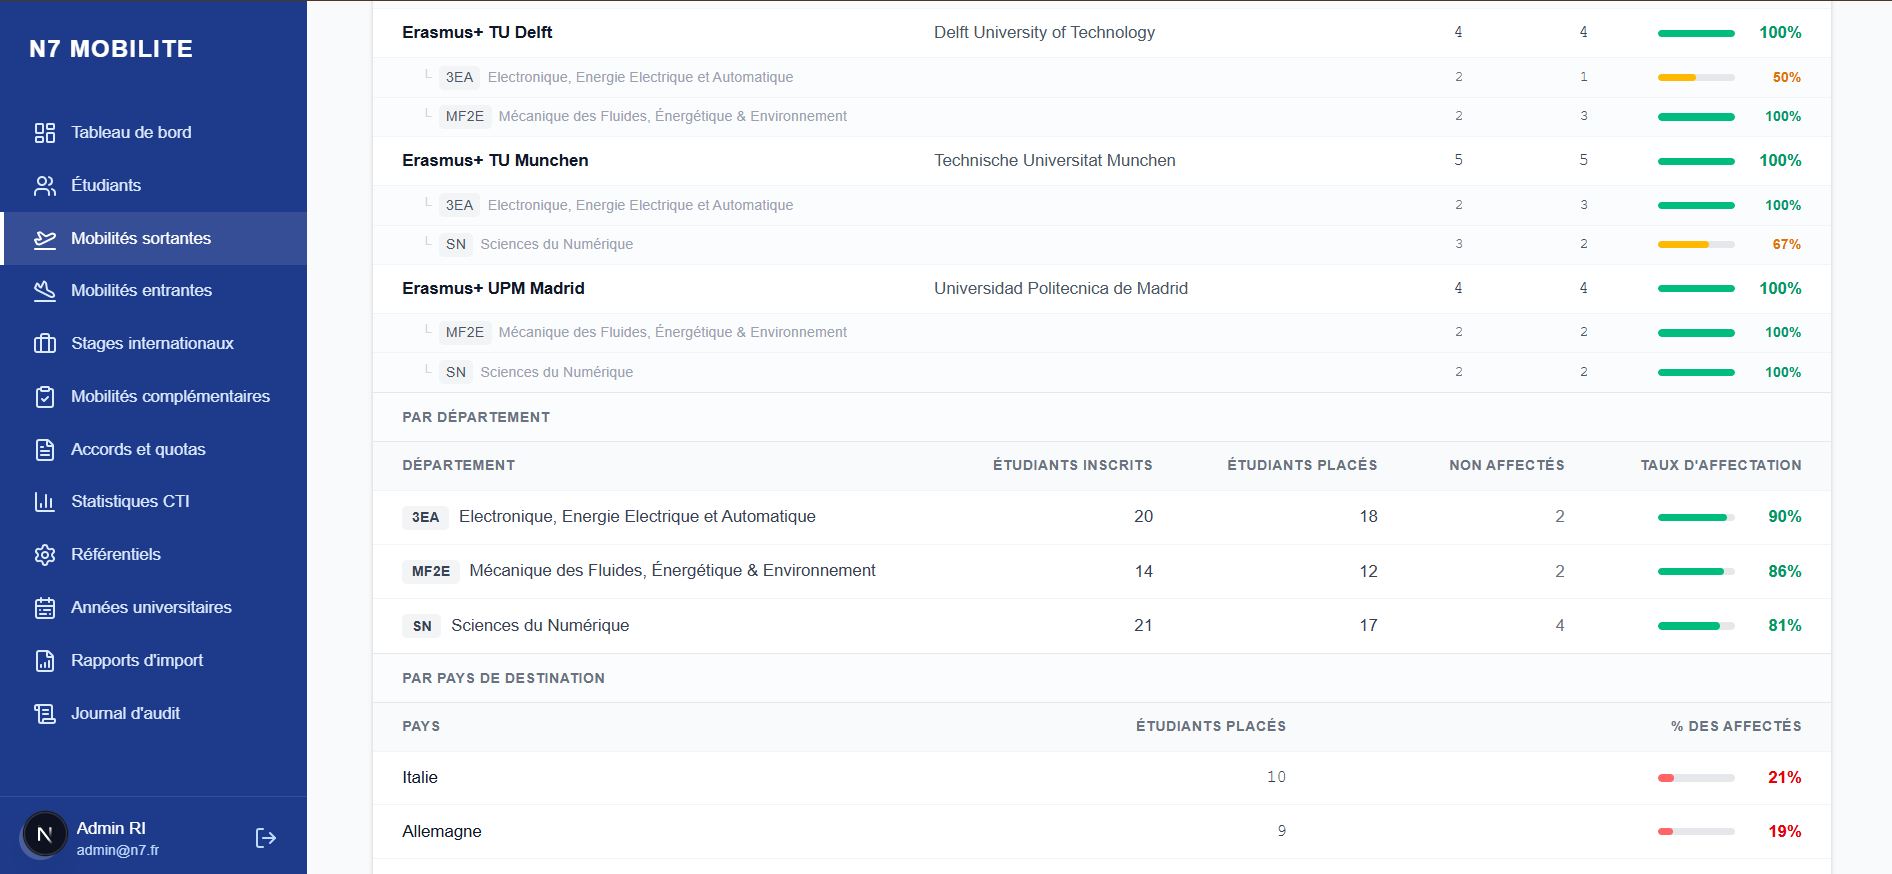
\includegraphics[width=\linewidth]{figures/captures/sprint3/sprint3-statistiques.png}
  \caption{Statistiques détaillées de l'affectation}
  \label{fig:cap-sprint3-statistiques}
\end{figure}

\bigskip
\noindent\textbf{A.2~--- Sprint 4 : consultations et mobilités complémentaires}
\par\smallskip

\begin{figure}[H]
  \centering
  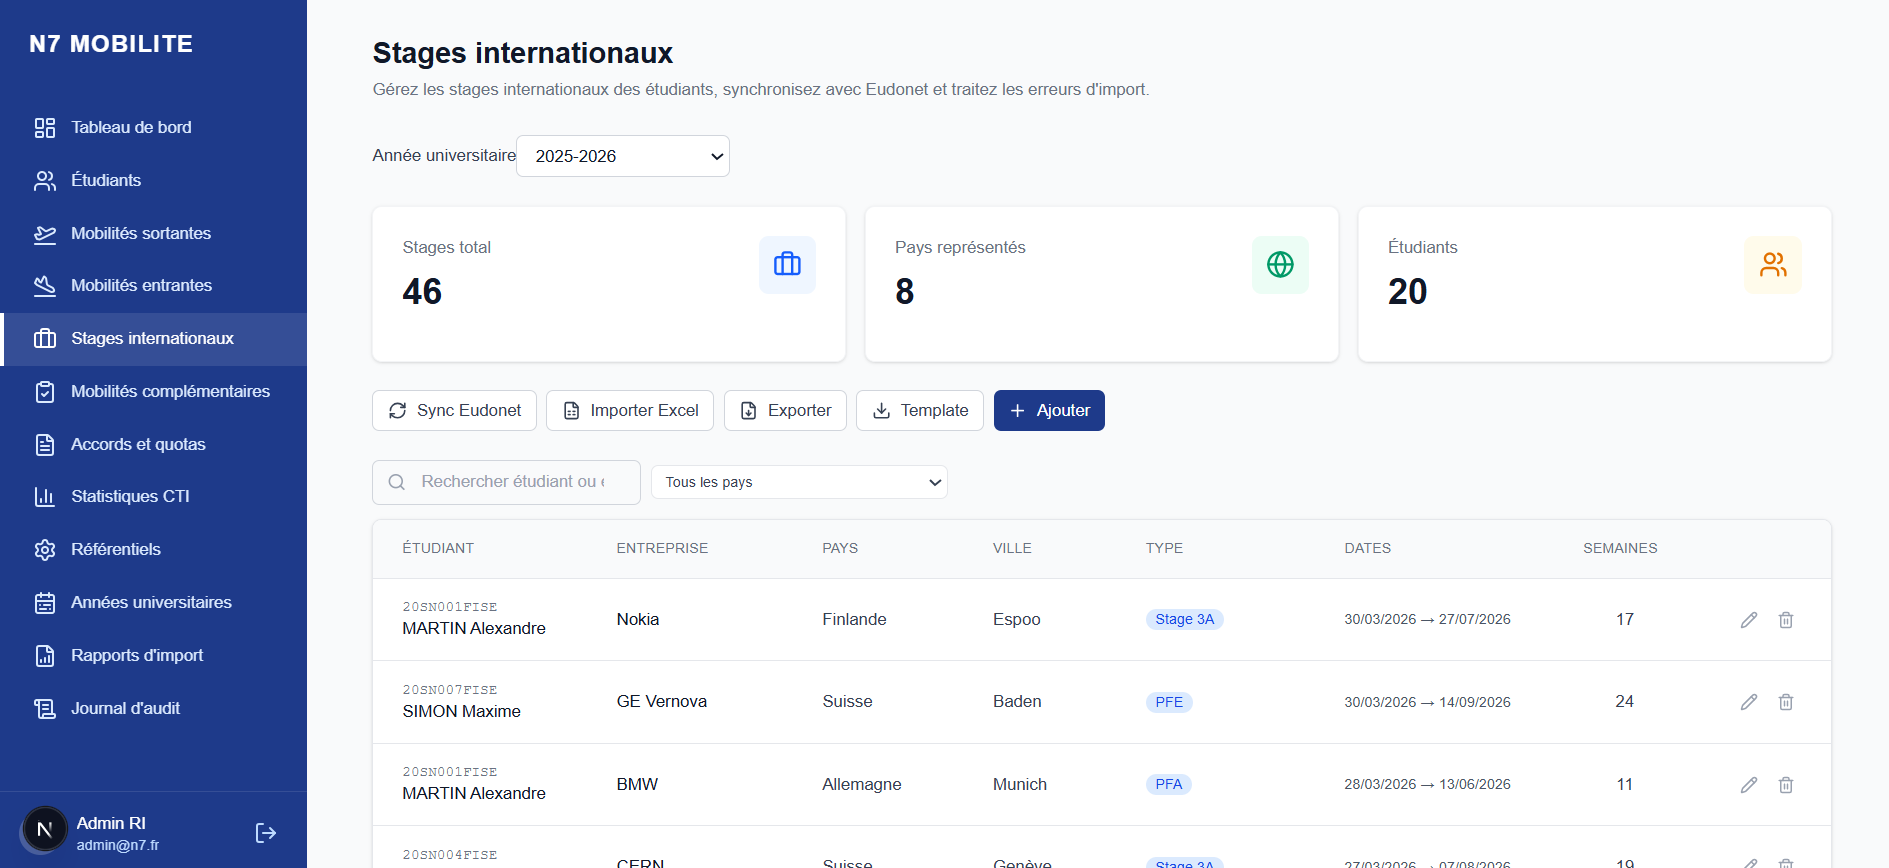
\includegraphics[width=0.85\linewidth]{figures/captures/sprint4/sprint4-stages.png}
  \caption{Consultation des stages internationaux}
  \label{fig:cap-sprint4-stages}
\end{figure}

\begin{figure}[H]
  \centering
  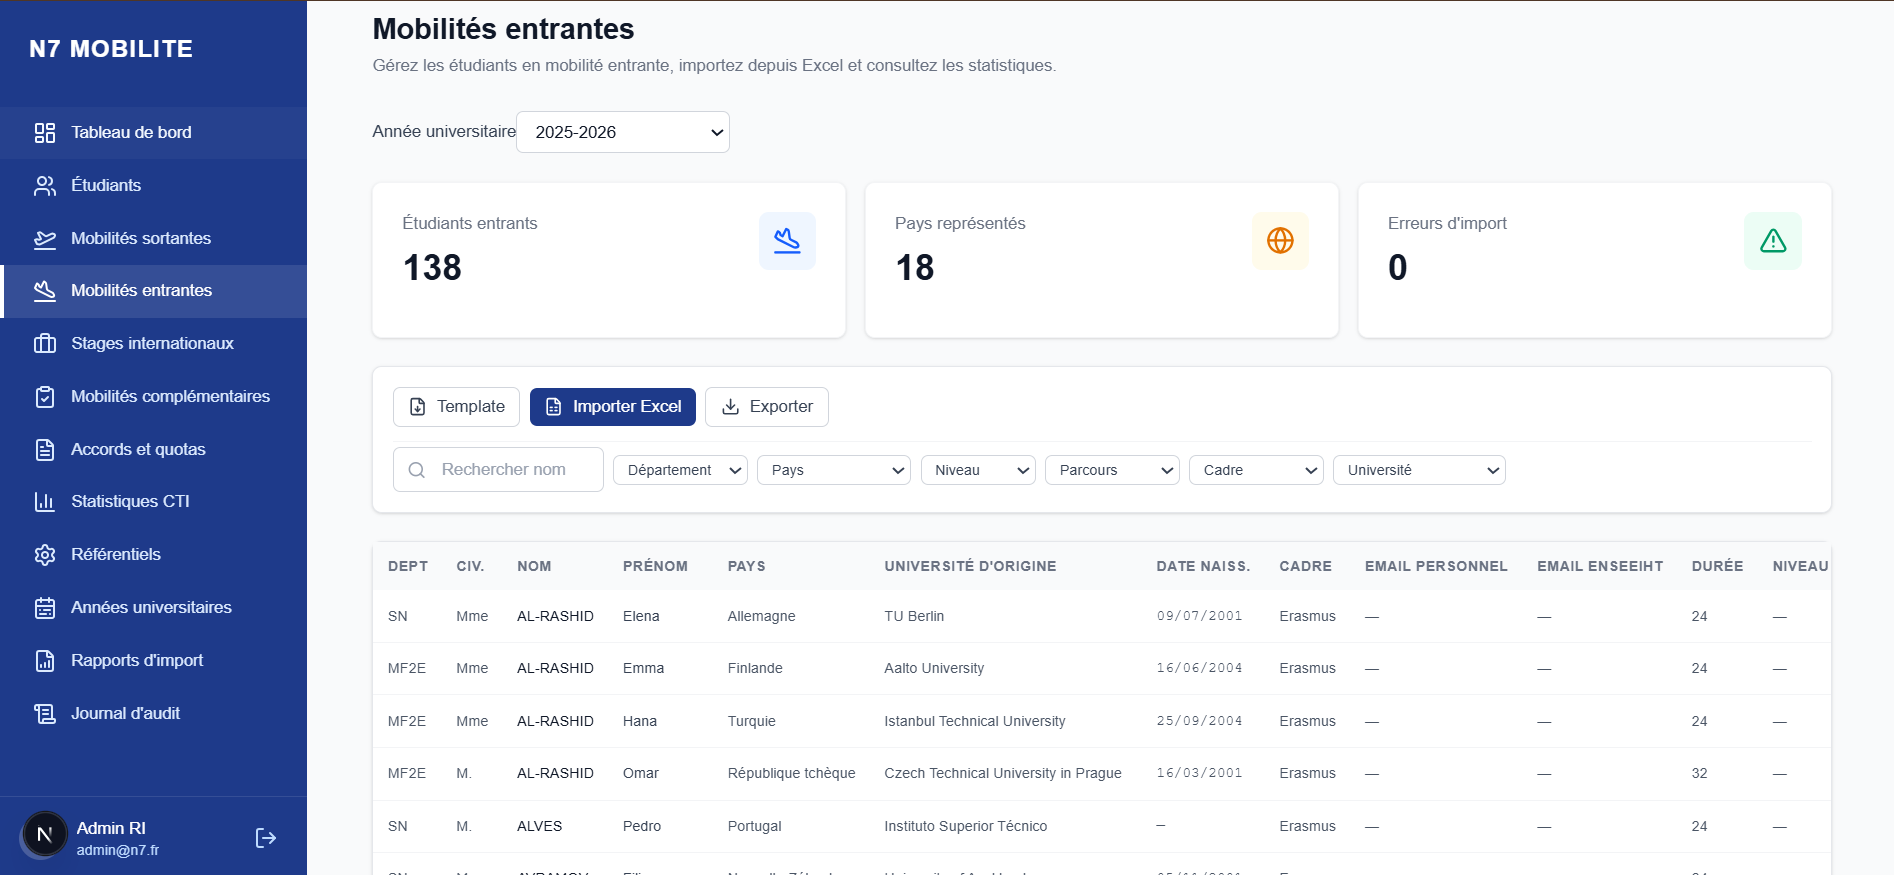
\includegraphics[width=0.85\linewidth]{figures/captures/sprint4/sprint4-entrantes.png}
  \caption{Consultation des mobilités entrantes}
  \label{fig:cap-sprint4-entrantes}
\end{figure}

\begin{figure}[H]
  \centering
  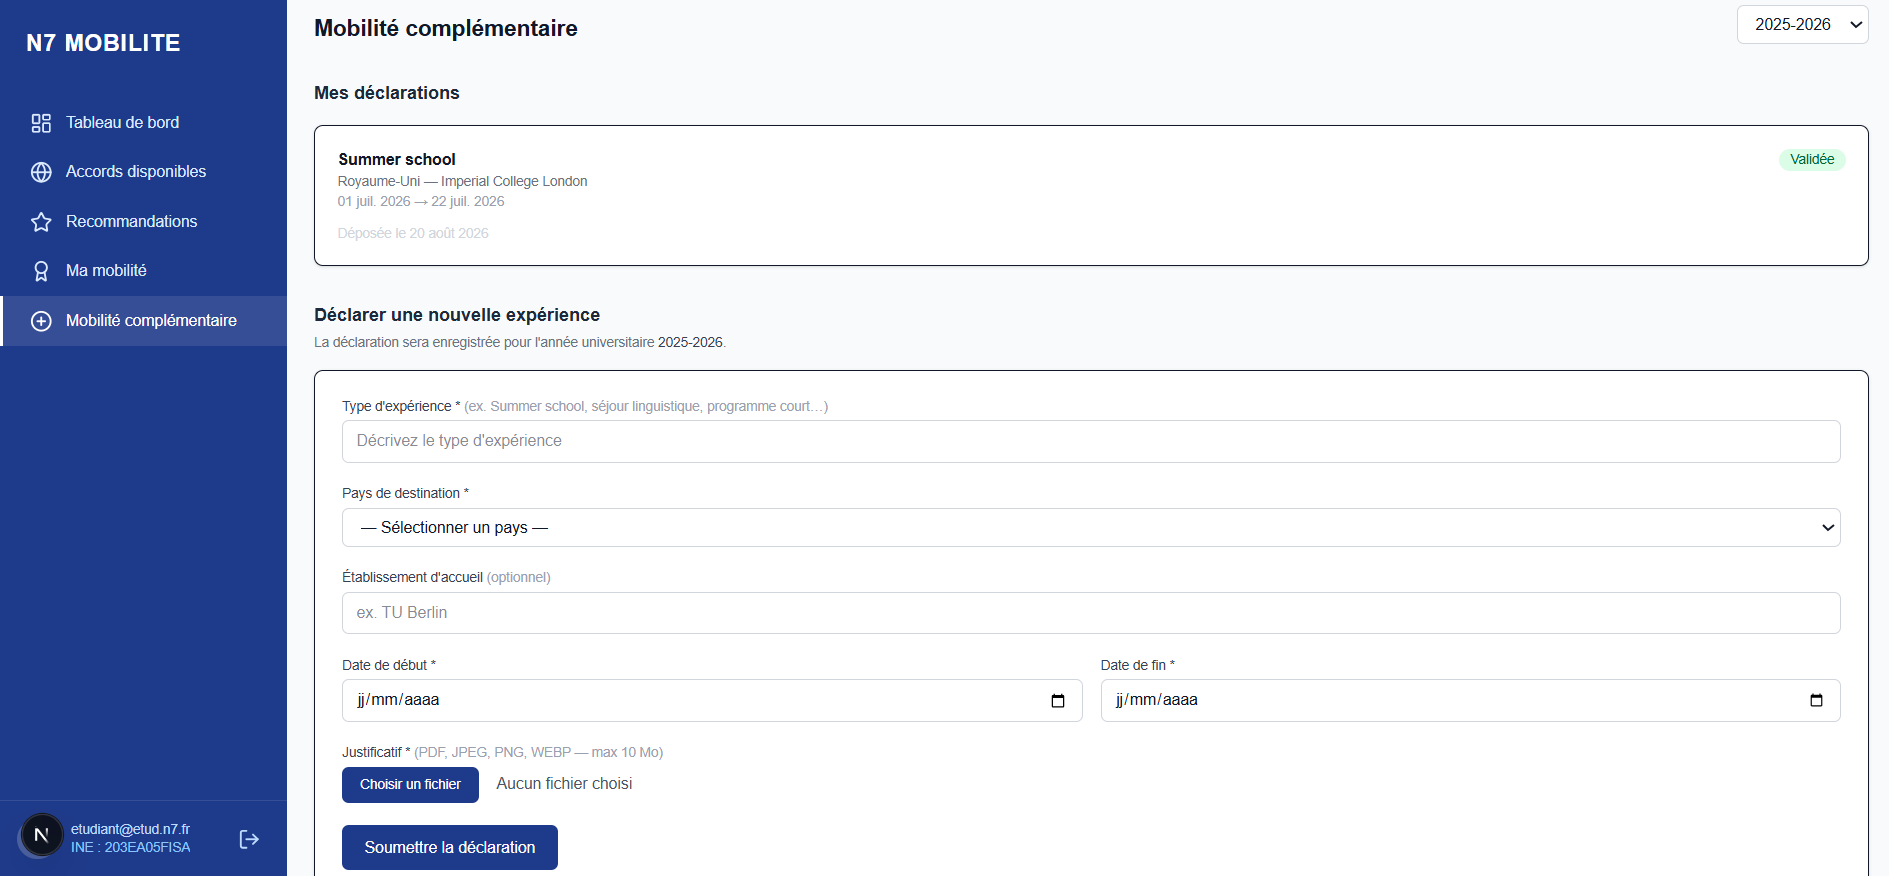
\includegraphics[width=0.85\linewidth]{figures/captures/sprint4/sprint4-declaration-etudiant.png}
  \caption{Déclaration d'une mobilité complémentaire (espace étudiant)}
  \label{fig:cap-sprint4-declaration}
\end{figure}

\begin{figure}[H]
  \centering
  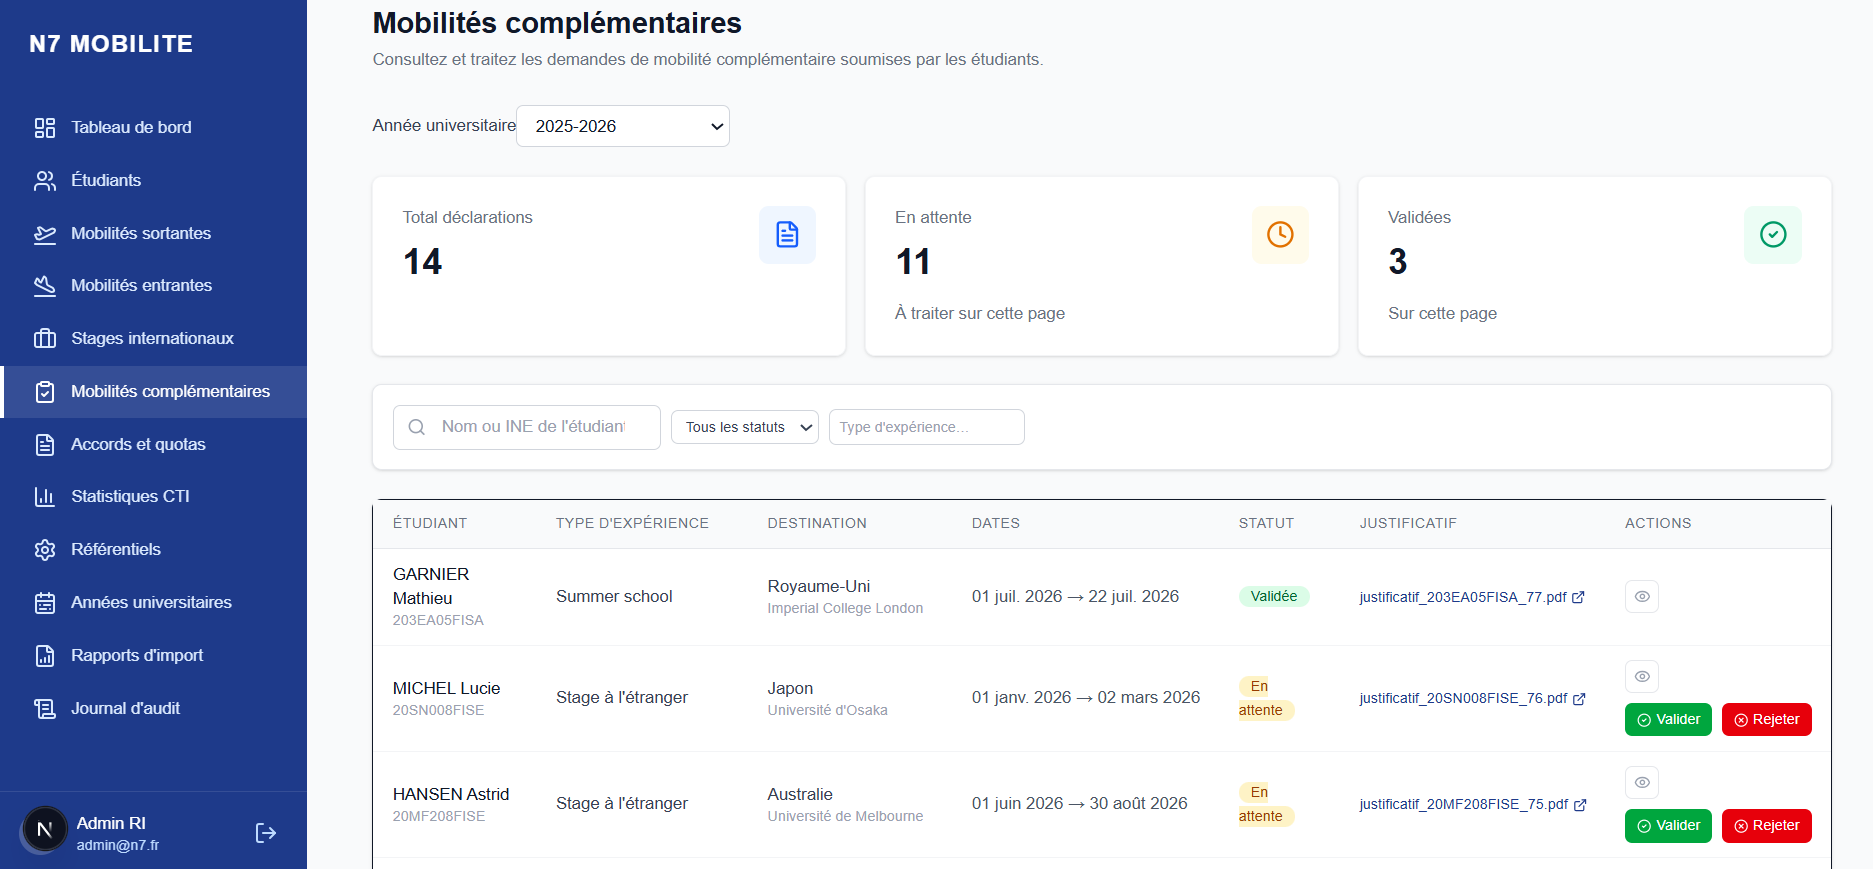
\includegraphics[width=0.85\linewidth]{figures/captures/sprint4/sprint4-mobilite-complementaire.png}
  \caption{Validation d'une mobilité complémentaire}
  \label{fig:cap-sprint4-mobilite-complementaire}
\end{figure}

\bigskip
\noindent\textbf{A.3~--- Sprint 5 : déclinaisons du tableau de bord analytique}
\par\smallskip

\begin{figure}[H]
  \centering
  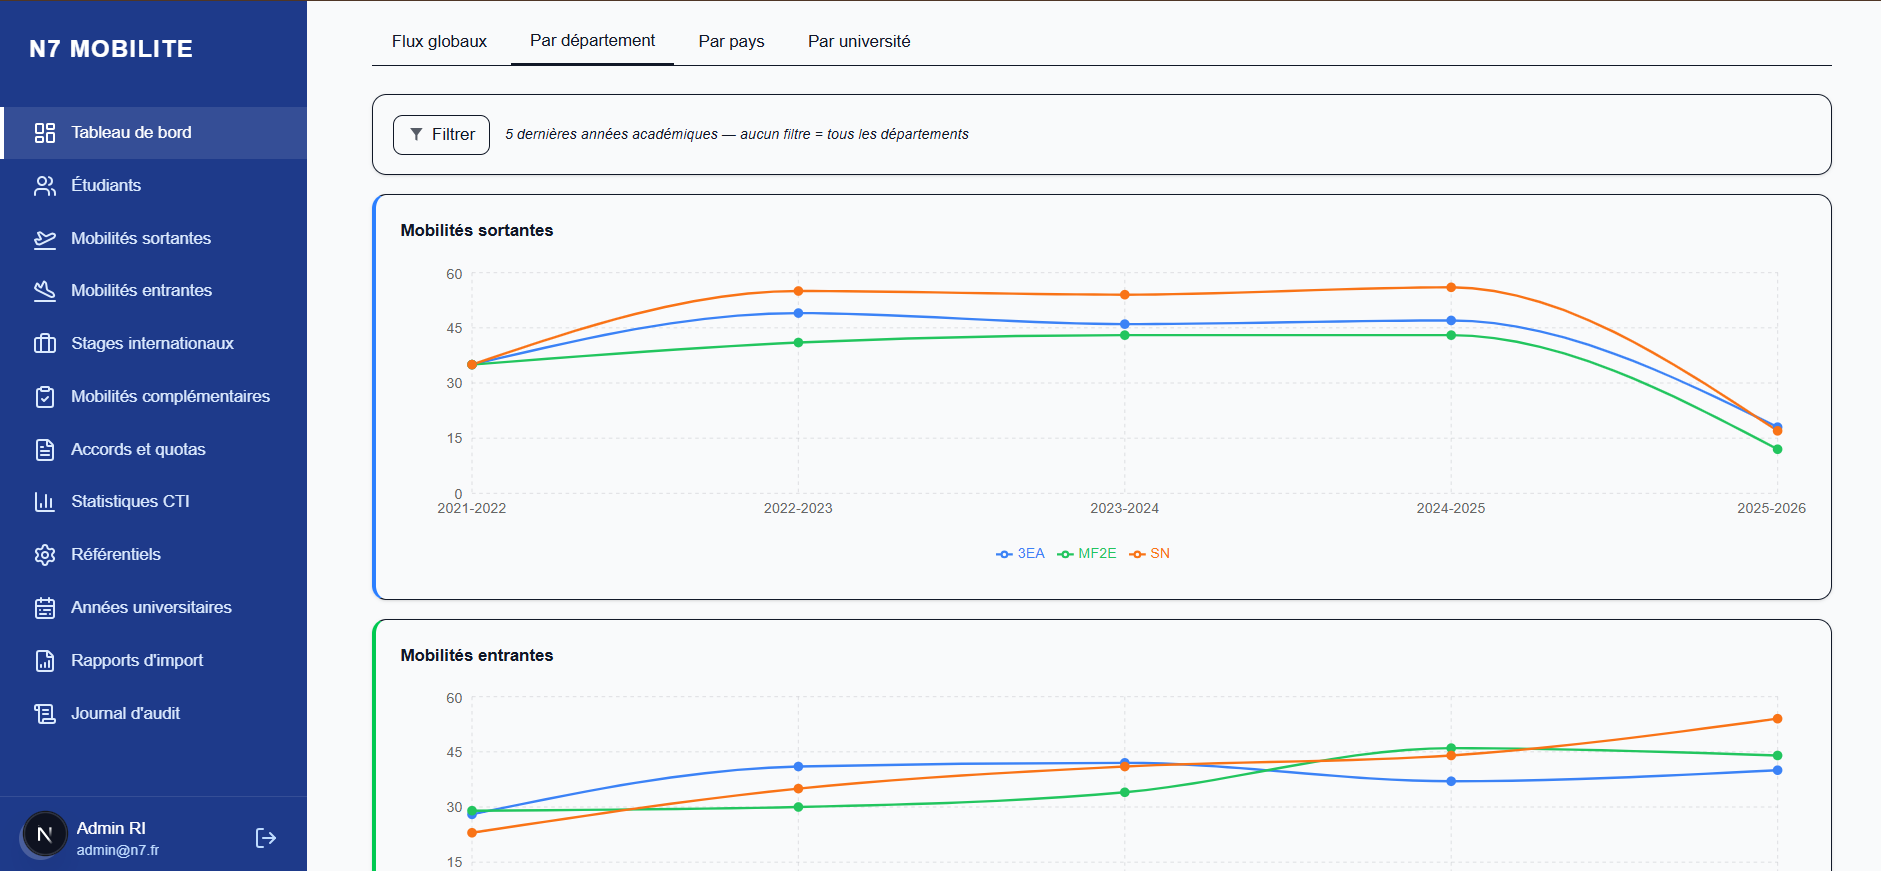
\includegraphics[width=0.85\linewidth]{figures/captures/sprint5/sprint5-dashboard-departement.png}
  \caption{Tableau de bord analytique : répartition par département}
  \label{fig:cap-sprint5-departement}
\end{figure}

\begin{figure}[H]
  \centering
  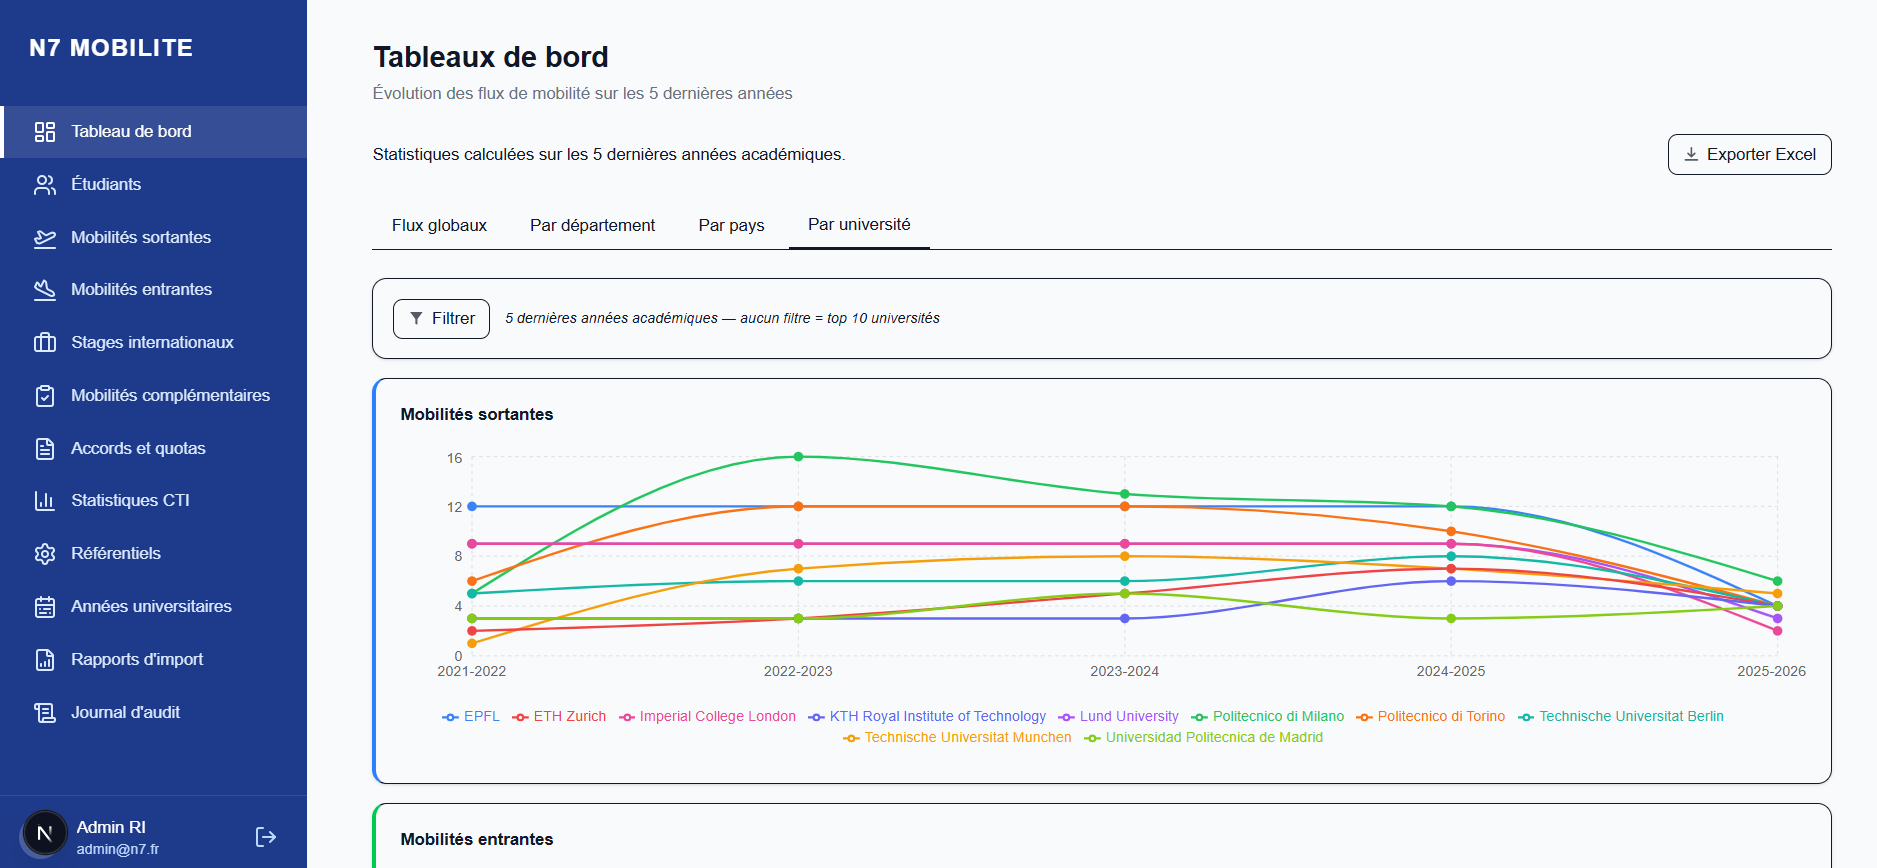
\includegraphics[width=0.85\linewidth]{figures/captures/sprint5/sprint5-dashboard-universite.png}
  \caption{Tableau de bord analytique : répartition par université partenaire}
  \label{fig:cap-sprint5-universite}
\end{figure}

\begin{figure}[H]
  \centering
  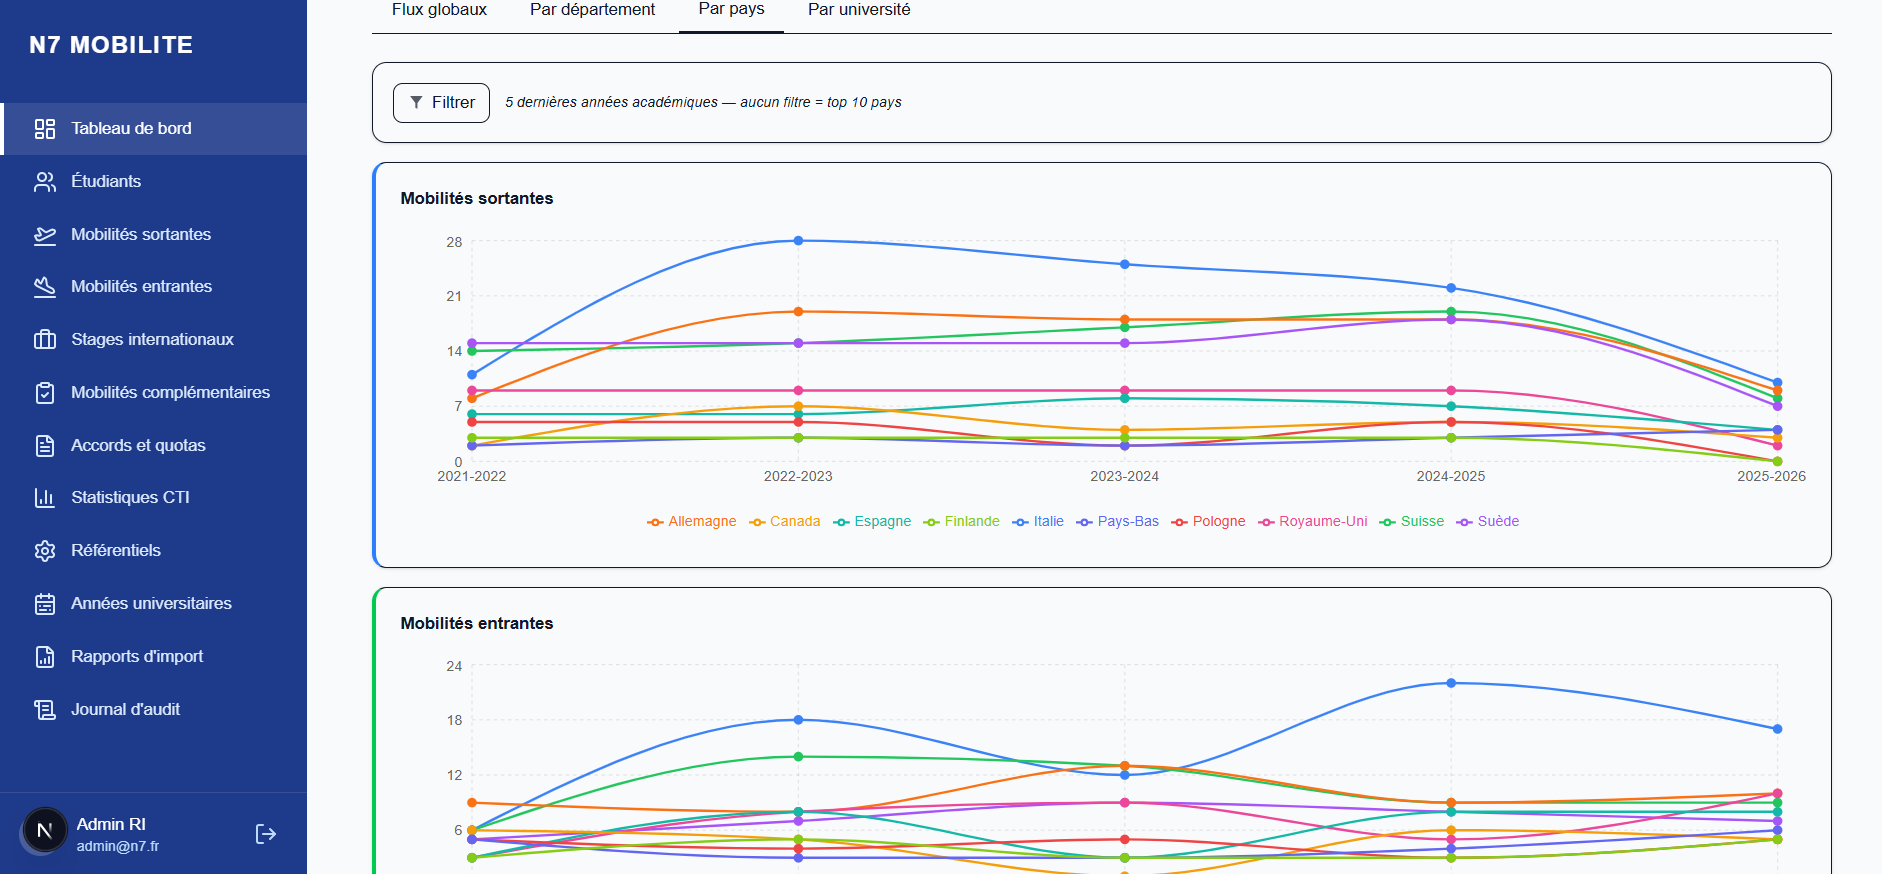
\includegraphics[width=0.85\linewidth]{figures/captures/sprint5/sprint5-dashboard-pays.png}
  \caption{Tableau de bord analytique : répartition par pays}
  \label{fig:cap-sprint5-pays}
\end{figure}
